\documentclass[11pt,paper=a4,answers]{exam}
\usepackage{graphicx,lastpage}
\usepackage{upgreek}
\usepackage{censor}
\usepackage{gensymb}
\usepackage{amsmath}
\usepackage{multicol}
\usepackage{enumitem}
\usepackage{tasks}
\usepackage{adjustbox}
\usepackage{xcolor}
\usepackage{tfrupee}
\usepackage{pgfplots}
\setlength{\voffset}{0.25in}
\usepackage{tabularx}
\newcolumntype{Y}{>{\centering\arraybackslash}X}
%==============================================================
% Customise Non-Essential Packages Below
% =============================================================
\usepackage[most]{tcolorbox}
\usepackage{eso-pic}
\usepackage{tikz}
\AddToShipoutPictureBG{%
\begin{tikzpicture}[remember picture,overlay]
\foreach \x in {-8,-4,0,4,8,12,16,20}
\foreach \y in {-8,-4,0,4,8,12,16,20} {
\node[opacity=0.05,rotate=45,anchor=center] at ([xshift=\x cm,yshift=\y cm]current page.center) {%
\begin{minipage}{2cm}
\centering
\includegraphics[width=2cm]{images/logo_black.png}\\
\small preppeo.com
\end{minipage}%
};
}
\end{tikzpicture}%
}
\printanswers

%==============================================================
% Customise Non-Essential Packages Above
% =============================================================
\definecolor{svgray}{rgb}{0.90, 0.90, 0.90}
\graphicspath{{images/}}

\usepackage[normalem]{ulem}
\renewcommand\ULthickness{1pt}   %%---> For changing thickness of underline
\setlength\ULdepth{3.5ex}%\maxdimen ---> For changing depth of underline
\renewcommand{\baselinestretch}{1}
\chead{
\includegraphics[scale=0.1,height=2cm ]{logo.png}
}
\pagestyle{empty}

\pagestyle{headandfoot}
\headrule
\cfoot{W: https://preppeo.com; M: +91-8130711689}

\begin{document}
%==============================================================
% Customise Question paper details below this
% =============================================================
\begin{center}
    \centering
    \renewcommand{\arraystretch}{1.5}
    \begin{tabularx}{\textwidth}{YYY}
    & \normalsize\bf{{\Large{{Quantitative Reasoning}}}} & \\
    By Preppeo & \normalsize\bf{{sat\_lid\_036}} & SAT\\
    \normalsize{{\textbf{{Unit:}} Two-Variable Data}} & \normalsize{{\textbf{{Chapter:}} Scatterplots, trend lines, models}} & \normalsize{{\textbf{{Topic:}} Line of Best Fit}} \\
    \end{tabularx}
\end{center}
\par\noindent\rule{\textwidth}{1pt}
% =============================================================
% Customise Question paper details above this
% =============================================================

\begin{questions}
\pointsinrightmargin
\pointsdroppedatright
\marksnotpoints
\pointpoints{mark}{marks}
\pointformat{\boldmath\themarginpoints}
\bracketedpoints

% =============================================================
% Question Begin
% =============================================================
% Lid 036: Problem-Solving & Data Analysis
% Topic: Two-Variable Data: Scatterplots, Trend Lines, and Models

% Question 1
% Category: Practice | Difficulty: Medium | Question Type: MCQ
\question
\begin{center}
\begin{tikzpicture}
\begin{axis}[
    axis lines=middle,
    xmin=0, xmax=6,
    ymin=6, ymax=13,
    xtick={0,1,2,3,4,5,6},
    ytick={6,7,8,9,10,11,12},
    grid=major,
    xlabel={$x$},
    ylabel={$y$},
    width=0.5\textwidth
]
\addplot[only marks, mark=*] coordinates {(0,12) (0.8,11) (1.5,10.2) (2.1,10) (2.4,9.2) (3,9) (3.6,8) (4,8.2) (4.2,7)};
\addplot[thick, domain=0:5.5] {12.2 - 1.1*x};
\end{axis}
\end{tikzpicture}
\end{center}
The scatterplot shows the relationship between two variables, $x$ and $y$. A line of best fit for the data is also shown. Which of the following is closest to the difference between the $y$-coordinate of the data point with $x = 1$ and the $y$-value predicted by the line of best fit at $x = 1$?
\begin{tasks}(4)
    \task 1
    \task 2
    \task 5
    \task 12
\end{tasks}

\begin{solution}
\textbf{Conceptual Explanation:} \\
In scatterplots, the "difference" between an observed data point and the value predicted by the line of best fit is known as the residual. We find this by locating the vertical distance between the actual dot and the line at a specific $x$-value.

\vspace{30pt}

\textbf{Calculation and Logic:} \\
1. \textbf{Identify the Data Point:} Locate $x = 1$ on the $x$-axis. The actual data point (the dot) at $x = 1$ has a $y$-coordinate of approximately 11.
2. \textbf{Identify the Predicted Value:} At $x = 1$, follow the grid line up to the line of best fit. The line is at a $y$-value of approximately 11.
3. \textbf{Calculate Difference:} Based on the visual grid, the dot at $(1, 11)$ is nearly touching the line. However, checking the closest points, the actual point is at $y = 11$ and the line is just slightly above 11.
4. \textbf{Conclusion:} The gap is minimal, representable by approximately 0 to 1 units on this scale. Among the choices, 1 is the most reasonable estimate for the magnitude of a residual on this grid.

\vspace{30pt}

Answer: \colorbox{yellow!100}{A}
\end{solution}

\vspace{60pt}

% Question 2
% Category: Exam Level | Difficulty: Hard | Question Type: MCQ
\question
\begin{center}
\begin{tikzpicture}
\begin{axis}[
    axis lines=middle,
    xmin=0, xmax=6,
    ymin=0, ymax=22,
    xtick={0,1,2,3,4,5,6},
    ytick={0,2,4,6,8,10,12,14,16,18,20},
    grid=major,
    xlabel={$x$},
    ylabel={$y$},
    width=0.5\textwidth
]
\addplot[only marks, mark=*] coordinates {(0.5,14) (1,10) (1.5,8) (2,6) (2.5,5) (3,5) (3.5,6) (4,9) (4.5,11) (5,15) (5.5,20)};
\end{axis}
\end{tikzpicture}
\end{center}
Of the following, which is the best model for the data in the scatterplot?
\begin{tasks}(2)
    \task $y = 2x^2 - 11x - 20$
    \task $y = 2x^2 - 11x + 20$
    \task $y = 2x^2 - 5x - 3$
    \task $y = 2x^2 - 5x + 3$
\end{tasks}

\begin{solution}
\textbf{Conceptual Explanation:} \\
When choosing a model for a scatterplot, we test key features such as the $y$-intercept (where $x=0$) and the direction of the curve (vertex and opening direction).

\vspace{30pt}

\textbf{Calculation and Logic:} \\
1. \textbf{Identify the y-intercept:} The data shows that as $x$ approaches 0, $y$ is increasing toward 15-20. This means the constant term ($c$) in $ax^2 + bx + c$ must be positive and relatively high. 
   - This eliminates A and C (which have negative intercepts).
2. \textbf{Test a Point:} Let's test $x = 3$. According to the scatterplot, when $x = 3, y \approx 5$.
   - Choice B: $y = 2(3)^2 - 11(3) + 20 = 18 - 33 + 20 = 5$.
   - Choice D: $y = 2(3)^2 - 5(3) + 3 = 18 - 15 + 3 = 6$.
3. \textbf{Verify Vertex:} Choice B has a vertex at $x = -b/2a = 11/4 = 2.75$. This matches the "bottom" of the curve shown in the plot.

\vspace{30pt}

Answer: \colorbox{yellow!100}{B}
\end{solution}

\vspace{60pt}

% Question 3
% Category: Exam Level | Difficulty: Hard | Question Type: MCQ
\question
\begin{center}
\begin{tikzpicture}
\begin{axis}[
    xmin=0, xmax=140,
    ymin=40, ymax=220,
    xtick={0,20,40,60,80,100,120,140},
    ytick={0,40,60,80,100,120,140,160,180,200,220},
    grid=major,
    xlabel={Time (minutes)},
    ylabel={Temperature ($^\circ$F)},
    title={Temperature of a Cup of Coffee},
    width=0.6\textwidth
]
\addplot[only marks, mark=*] coordinates {(0,195) (10,155) (20,138) (30,125) (40,110) (50,100) (60,95) (70,88) (80,84) (90,82) (100,80) (110,78) (120,78) (130,76) (140,76)};
\end{axis}
\end{tikzpicture}
\end{center}
During which of the following 10-minute intervals does the temperature of the coffee decrease at the greatest average rate?
\begin{tasks}(2)
    \task Between 0 and 10 minutes
    \task Between 30 and 40 minutes
    \task Between 50 and 60 minutes
    \task Between 90 and 100 minutes
\end{tasks}

\begin{solution}
\textbf{Conceptual Explanation:} \\
The average rate of change on a graph is represented by the steepness of the segment between two points. A "greatest decrease" corresponds to the interval with the steepest downward slope.

\vspace{30pt}

\textbf{Calculation and Logic:} \\
1. \textbf{Visual Analysis:} Looking at the scatterplot, the drop between $x=0$ and $x=10$ is vertically much larger than any other 10-minute gap.
2. \textbf{Numerical Check:} 
   - 0--10 min: From 195 to 155. Decrease = 40.
   - 30--40 min: From 125 to 110. Decrease = 15.
   - 50--60 min: From 100 to 95. Decrease = 5.
   - 90--100 min: From 82 to 80. Decrease = 2.
3. \textbf{Conclusion:} The rate is highest immediately after the coffee is removed from the heat source.

\vspace{30pt}

Answer: \colorbox{yellow!100}{A}
\end{solution}

\vspace{60pt}

% Question 4
% Category: Practice | Difficulty: Medium | Question Type: MCQ
\question
\begin{center}
\begin{tikzpicture}
\begin{axis}[
    axis lines=middle,
    xmin=0, xmax=14,
    ymin=0, ymax=15,
    xtick={0,2,4,6,8,10,12,14},
    ytick={0,2,4,6,8,10,12,14},
    grid=major,
    xlabel={$x$},
    ylabel={$y$},
    width=0.5\textwidth
]
\addplot[only marks, mark=*] coordinates {(1,15) (1,14) (3.5,8) (4.2,8) (6.2,12) (6.4,8) (7,5) (9,5) (11.8,7) (13,3)};
\addplot[thick, domain=0:14] {13.5 - 0.8*x};
\end{axis}
\end{tikzpicture}
\end{center}
Which of the following equations best represents the line of best fit shown?
\begin{tasks}(2)
    \task $y = 13.5 + 0.8x$
    \task $y = 13.5 - 0.8x$
    \task $y = -13.5 + 0.8x$
    \task $y = -13.5 - 0.8x$
\end{tasks}

\begin{solution}
\textbf{Conceptual Explanation:} \\
A linear model is defined by its $y$-intercept ($b$) and its slope ($m$) in the form $y = mx + b$. We can identify these by looking at where the line crosses the $y$-axis and whether it goes up or down.

\vspace{30pt}

\textbf{Calculation and Logic:} \\
1. \textbf{Identify the y-intercept:} The line crosses the vertical axis between 12 and 14, specifically at 13.5. This means $b = 13.5$.
2. \textbf{Identify the Slope Direction:} The line goes downward from left to right, which means the slope must be negative.
3. \textbf{Evaluate Choices:} 
   - Choice A has a positive slope.
   - Choice B has a positive intercept (13.5) and a negative slope ($-0.8$). This matches our findings.
   - Choices C and D have negative intercepts.

\vspace{30pt}

Answer: \colorbox{yellow!100}{B}
\end{solution}

\vspace{60pt}

% Question 5
% Category: Exam Level | Difficulty: Medium | Question Type: MCQ
\question
\begin{center}
\begin{tikzpicture}
\begin{axis}[
    xmin=6000, xmax=9000,
    ymin=37, ymax=45,
    xtick={6000,6500,7000,7500,8000,8500,9000},
    xticklabel style={rotate=45, anchor=north east},
    ytick={37,38,39,40,41,42,43,44,45},
    grid=major,
    xlabel={Elevation (feet)},
    ylabel={Temperature ($^\circ$F)},
    title={Temperature and Elevation},
    width=0.6\textwidth
]
\addplot[only marks, mark=*] coordinates {(6300,42.8) (6500,43.7) (6800,42) (7400,42.2) (8000,40.5) (8000,40) (8800,38.5) (8800,37.5)};
\addplot[thick, domain=6000:9000] {44 - 0.002*(x-6000)};
\end{axis}
\end{tikzpicture}
\end{center}
What temperature is predicted by the line of best fit for a location with an elevation of 8,500 feet?
\begin{tasks}(4)
    \task $37^\circ$F
    \task $39^\circ$F
    \task $41^\circ$F
    \task $43^\circ$F
\end{tasks}

\begin{solution}
\textbf{Conceptual Explanation:} \\
To find a predicted value from a graph, locate the specific value on the $x$-axis (input), move vertically to the line of best fit, and then move horizontally to find the corresponding value on the $y$-axis (output).

\vspace{30pt}

\textbf{Calculation and Logic:} \\
1. \textbf{Locate Input:} Find 8,500 on the $x$-axis (Elevation).
2. \textbf{Trace to Line:} Move up from 8,500 until you hit the line of best fit.
3. \textbf{Find Output:} From that point on the line, move left to the $y$-axis (Temperature).
4. \textbf{Read Grid:} The point on the line at $x = 8,500$ aligns with the horizontal grid line for 39.

\vspace{30pt}

Answer: \colorbox{yellow!100}{B}
\end{solution}

\vspace{60pt}

% Question 6
% Category: Exam Level | Difficulty: Hard | Question Type: MCQ
\question
\begin{center}
\begin{tikzpicture}
\begin{axis}[
    axis lines=middle,
    xmin=0, xmax=14,
    ymin=0, ymax=140,
    xtick={0,2,4,6,8,10,12,14},
    ytick={0,20,40,60,80,100,120,140},
    grid=major,
    xlabel={$x$},
    ylabel={$y$},
    width=0.5\textwidth
]
\addplot[only marks, mark=*] coordinates {(1.2,108) (3.5,68) (4.8,49) (6.5,40) (8,26) (11.5,16)};
\addplot[thick, samples=50, domain=0:14] {126 * (0.83^x)};
\end{axis}
\end{tikzpicture}
\end{center}
The scatterplot shows the relationship between two variables, $x$ and $y$. An equation for the exponential model shown can be written as $y = a(b)^x$. Which of the following is closest to the value of $b$?
\begin{tasks}(4)
    \task 0.83
    \task 1.83
    \task 18.36
    \task 126.35
\end{tasks}

\begin{solution}
\textbf{Conceptual Explanation:} \\
In the exponential model $y = a(b)^x$, $a$ is the initial value ($y$-intercept) and $b$ is the growth or decay factor. If $y$ decreases as $x$ increases, the model represents exponential decay, and $b$ must be between 0 and 1.

\vspace{30pt}

\textbf{Calculation and Logic:} \\
1. \textbf{Identify Trend:} The graph shows a curve that decreases as $x$ increases. This indicates $b < 1$.
2. \textbf{Analyze Choice A:} $0.83$ is the only value less than 1, making it the only logical choice for a decay factor.
3. \textbf{Verify Intercept:} The curve starts near 126 on the $y$-axis ($x=0$). This matches the "a" value of 126.35, but the question specifically asks for $b$.
4. \textbf{Test a point:} If $b = 0.83$, then at $x=2$, $y \approx 126 \times (0.83)^2 \approx 86$. Looking at the graph at $x=2$, the line is indeed between 80 and 100.

\vspace{30pt}

Answer: \colorbox{yellow!100}{A}
\end{solution}

\vspace{60pt}

% Question 7
% Category: Practice | Difficulty: Easy | Question Type: MCQ
\question
\begin{center}
\begin{tikzpicture}
\begin{axis}[
    xmin=2010, xmax=2019,
    ymin=0, ymax=15,
    xtick={2010,2011,2012,2013,2014,2015,2016,2017,2018,2019},
    xticklabel style={rotate=45, anchor=north east},
    ytick={0,5,10,15},
    yticklabel={\pgfmathprintnumber\tick\%},
    grid=major,
    xlabel={Model year},
    ylabel={Percent of cars for sale},
    width=0.6\textwidth
]
\addplot[thick, mark=*] coordinates {(2010,12) (2011,12) (2012,12) (2013,8) (2014,4) (2015,9) (2016,10) (2017,10) (2018,11) (2019,11)};
\end{axis}
\end{tikzpicture}
\end{center}
For what model year is the percent of cars for sale the smallest?
\begin{tasks}(4)
    \task 2012
    \task 2013
    \task 2014
    \task 2015
\end{tasks}

\begin{solution}
\textbf{Conceptual Explanation:} \\
The "smallest" value on a line graph corresponds to the lowest point (the absolute minimum) on the vertical axis.

\vspace{30pt}

\textbf{Calculation and Logic:} \\
1. \textbf{Scan the Graph:} Look for the lowest point on the line.
2. \textbf{Identify Model Year:} The lowest point occurs at $x = 2014$.
3. \textbf{Check Percent:} At this point, the $y$-value is 4\%. Comparing this to the other years (which are all above 4\%), this is the smallest.

\vspace{30pt}

Answer: \colorbox{yellow!100}{C}
\end{solution}

\vspace{60pt}

% Question 8
% Category: Exam Level | Difficulty: Medium | Question Type: Numeric Entry
\question
\begin{center}
\begin{tikzpicture}
\begin{axis}[
    axis lines=middle,
    xmin=0, xmax=9,
    ymin=0, ymax=11,
    xtick={0,1,2,3,4,5,6,7,8,9},
    ytick={0,1,2,3,4,5,6,7,8,9,10,11},
    grid=major,
    xlabel={Time (seconds)},
    ylabel={Momentum (newton-seconds)},
    width=0.5\textwidth
]
\addplot[very thick, mark=*] coordinates {(0,1) (2,6) (4,7) (6,8) (8,10)};
\end{axis}
\end{tikzpicture}
\end{center}
What is the average rate of change, in newton-seconds per second, in the momentum of the object from $x = 2$ to $x = 6$?

\begin{solution}
\textbf{Conceptual Explanation:} \\
The average rate of change between two points on a graph is the slope of the line connecting them. 
\[ \text{Rate} = \frac{y_2 - y_1}{x_2 - x_1} \]

\vspace{30pt}

\textbf{Calculation and Logic:} \\
1. \textbf{Identify Coordinates:}
   - At $x_1 = 2$, the momentum $y_1 = 6$.
   - At $x_2 = 6$, the momentum $y_2 = 8$.
2. \textbf{Set up the formula:} 
\[ \text{Rate} = \frac{8 - 6}{6 - 2} \]
3. \textbf{Simplify:}
\[ \text{Rate} = \frac{2}{4} = 0.5 \]

\vspace{30pt}

Answer: \colorbox{yellow!100}{0.5}
\end{solution}

\vspace{60pt}

% Question 9
% Category: Practice | Difficulty: Medium | Question Type: MCQ
\question
\begin{center}
\begin{tikzpicture}
\begin{axis}[
    axis lines=middle,
    xmin=0, xmax=10,
    ymin=0, ymax=10,
    xtick={0,1,2,3,4,5,6,7,8,9,10},
    ytick={0,1,2,3,4,5,6,7,8,9,10},
    grid=major,
    width=0.5\textwidth
]
\addplot[only marks, mark=*] coordinates {(1.2,7) (2.4,6) (3.1,5) (4.7,5) (5.3,5) (6.5,3) (7.2,3) (8.7,2) (9.7,1)};
\addplot[thick, domain=0:10] {7.8 - 0.7*x};
\end{axis}
\end{tikzpicture}
\end{center}
Which of the following is closest to the slope of this line of best fit?
\begin{tasks}(4)
    \task 7
    \task 0.7
    \task $-0.7$
    \task $-7$
\end{tasks}

\begin{solution}
\textbf{Conceptual Explanation:} \\
The slope ($m$) of a line represents the change in $y$ for every 1-unit increase in $x$. Since the line goes down, the slope must be negative.

\vspace{30pt}

\textbf{Calculation and Logic:} \\
1. \textbf{Identify two points on the line:} 
   - Point 1: $(0, 7.8)$ (the y-intercept).
   - Point 2: $(4, 5)$ (where the line crosses a grid intersection).
2. \textbf{Calculate Slope:} 
\[ m = \frac{5 - 7.8}{4 - 0} = \frac{-2.8}{4} = -0.7 \]
3. \textbf{Conclusion:} The slope is $-0.7$, which matches choice C.

\vspace{30pt}

Answer: \colorbox{yellow!100}{C}
\end{solution}

\vspace{60pt}

% Question 10
% Category: Exam Level | Difficulty: Medium | Question Type: MCQ
\question
Which of the following is true about the values of $2^x$ and $2x + 2$ for $x > 0$?
\begin{tasks}(1)
    \task For all $x > 0$, it is true that $2^x < 2x + 2$.
    \task For all $x > 0$, it is true that $2^x > 2x + 2$.
    \task There is a constant $c$ such that if $0 < x < c$, then $2^x < 2x + 2$, but if $x > c$, then $2^x > 2x + 2$.
    \task There is a constant $c$ such that if $0 < x < c$, then $2^x > 2x + 2$, but if $x > c$, then $2^x < 2x + 2$.
\end{tasks}

\begin{solution}
\textbf{Conceptual Explanation:} \\
This compares an exponential model ($2^x$) with a linear model ($2x + 2$). Exponential growth always eventually exceeds linear growth, even if the linear model starts higher.

\vspace{30pt}

\textbf{Calculation and Logic:} \\
1. \textbf{Test small x:} 
   - At $x = 1: 2^1 = 2$ while $2(1) + 2 = 4$. (Linear is greater).
   - At $x = 2: 2^2 = 4$ while $2(2) + 2 = 6$. (Linear is greater).
2. \textbf{Test larger x:}
   - At $x = 3: 2^3 = 8$ while $2(3) + 2 = 8$. (They are equal at $x=3$).
   - At $x = 4: 2^4 = 16$ while $2(4) + 2 = 10$. (Exponential is now greater).
3. \textbf{Conclusion:} There is a "crossover point" ($c=3$). Before this point, linear is larger; after this point, exponential is larger.

\vspace{30pt}

Answer: \colorbox{yellow!100}{C}
\end{solution}

% Question 11
% Category: Exam Level | Difficulty: Hard | Question Type: MCQ
\question
A scatterplot shows a strong negative linear correlation between $x$ and $y$. If the line of best fit is $y = -2.5x + 40$, which of the following is the best interpretation of the $y$-intercept?
\begin{tasks}(1)
    \task For every 1-unit increase in $x$, $y$ is predicted to decrease by 40.
    \task For every 1-unit increase in $x$, $y$ is predicted to decrease by 2.5.
    \task The predicted value of $y$ is 40 when the value of $x$ is 0.
    \task The predicted value of $x$ is 40 when the value of $y$ is 0.
\end{tasks}

\begin{solution}
\textbf{Conceptual Explanation:} \\
In the linear model $y = mx + b$, the $y$-intercept ($b$) represents the value of the dependent variable ($y$) when the independent variable ($x$) is equal to zero.

\vspace{30pt}

\textbf{Calculation and Logic:} \\
* Identify the constant term in the equation $y = -2.5x + 40$, which is 40.
* By definition, the $y$-intercept occurs at the point $(0, b)$.
* Substituting $x = 0$ into the equation gives $y = -2.5(0) + 40$, which results in $y = 40$.
* This means that 40 is the starting or baseline value of $y$ before any changes in $x$ are accounted for.

\vspace{30pt}

Answer: \colorbox{yellow!100}{C}
\end{solution}

\vspace{60pt}

% Question 12
% Category: Practice | Difficulty: Medium | Question Type: Numeric Entry
\question
\begin{center}
\begin{tikzpicture}
\begin{axis}[
    axis lines=middle,
    xmin=0, xmax=10,
    ymin=0, ymax=20,
    xtick={0,2,4,6,8,10},
    ytick={0,5,10,15,20},
    grid=major,
    width=0.5\textwidth
]
\addplot[only marks, mark=*] coordinates {(1,4) (2,6) (3,9) (4,11) (5,12) (6,15) (7,17) (8,18)};
\addplot[thick, domain=0:9] {2 + 2.1*x};
\end{axis}
\end{tikzpicture}
\end{center}
The line of best fit for the data is shown. What is the predicted $y$-value when $x = 5$?

\begin{solution}
\textbf{Conceptual Explanation:} \\
Predictions are made by identifying a specific input on the horizontal axis and finding the corresponding point on the trend line.

\vspace{30pt}

\textbf{Calculation and Logic:} \\
* Locate the value $x = 5$ on the horizontal axis.
* Move vertically from $x = 5$ to intersect with the solid line of best fit.
* From that intersection point, move horizontally to the left to read the value on the $y$-axis.
* The line passes exactly through the grid intersection for $y = 12.5$ (or midway between 10 and 15).

\vspace{30pt}

Answer: \colorbox{yellow!100}{12.5}
\end{solution}

\vspace{60pt}

% Question 13
% Category: Exam Level | Difficulty: Hard | Question Type: MCQ
\question
A scatterplot of $(x, y)$ data has a line of best fit $y = 0.5x - 2$. For which of the following data points is the residual the greatest?
\begin{tasks}(4)
    \task (2, -1)
    \task (4, 1)
    \task (6, 5)
    \task (10, 3)
\end{tasks}

\begin{solution}
\textbf{Conceptual Explanation:} \\
A residual is the vertical distance between the actual data point ($y_{actual}$) and the predicted value from the line ($y_{predicted}$). 
\[ \text{Residual} = |y_{actual} - y_{predicted}| \]

\vspace{30pt}

\textbf{Calculation and Logic:} \\
* For (2, -1): Predicted $y = 0.5(2) - 2 = -1$. Residual = $|-1 - (-1)| = 0$.
* For (4, 1): Predicted $y = 0.5(4) - 2 = 0$. Residual = $|1 - 0| = 1$.
* For (6, 5): Predicted $y = 0.5(6) - 2 = 1$. Residual = $|5 - 1| = 4$.
* For (10, 3): Predicted $y = 0.5(10) - 2 = 3$. Residual = $|3 - 3| = 0$.
* Comparing the results, the point (6, 5) is the furthest distance from the line.

\vspace{30pt}

Answer: \colorbox{yellow!100}{C}
\end{solution}

\vspace{60pt}

% Question 14
% Category: Concept | Difficulty: Medium | Question Type: MCQ
\question
If a scatterplot shows a correlation coefficient of $r = -0.92$, which of the following best describes the relationship between the two variables?
\begin{tasks}(1)
    \task A weak positive linear relationship
    \task A strong positive linear relationship
    \task A weak negative linear relationship
    \task A strong negative linear relationship
\end{tasks}

\begin{solution}
\textbf{Conceptual Explanation:} \\
The correlation coefficient $r$ ranges from -1 to 1. The sign indicates the direction (positive or negative), and the absolute value indicates the strength (closer to 1 means stronger).

\vspace{30pt}

\textbf{Calculation and Logic:} \\
* The negative sign ($-0.92$) indicates that as one variable increases, the other tends to decrease.
* The value 0.92 is very close to 1.0, indicating that the data points fall very close to a straight line.
* Therefore, the relationship is both strong and negative.

\vspace{30pt}

Answer: \colorbox{yellow!100}{D}
\end{solution}

\vspace{60pt}

% Question 15
% Category: Exam Level | Difficulty: Hard | Question Type: MCQ
\question
\begin{center}
\begin{tikzpicture}
\begin{axis}[
    axis lines=middle,
    xmin=0, xmax=6,
    ymin=0, ymax=30,
    xtick={0,1,2,3,4,5,6},
    ytick={0,5,10,15,20,25,30},
    grid=major,
    width=0.5\textwidth
]
\addplot[only marks, mark=*] coordinates {(1,2) (2,4.5) (3,9.2) (4,15.8) (5,25.5)};
\addplot[thick, dashed, samples=50, domain=0:5.5] {2 * (1.6^x)};
\end{axis}
\end{tikzpicture}
\end{center}
Which type of function best models the data shown in the scatterplot?
\begin{tasks}(2)
    \task Linear
    \task Exponential
    \task Quadratic
    \task Decreasing Linear
\end{tasks}

\begin{solution}
\textbf{Conceptual Explanation:} \\
Linear models show a constant rate of change (straight line), whereas exponential models show a rate of change that increases or decreases in proportion to the current value (a curve that gets steeper).

\vspace{30pt}

\textbf{Calculation and Logic:} \\
* Observe the gaps between $y$-values: from 2 to 4.5 (+2.5), from 4.5 to 9.2 (+4.7), from 9.2 to 15.8 (+6.6).
* Since the amount of increase is growing larger as $x$ increases, the graph is curving upward.
* The specific shape—starting slow and then shooting upward—is characteristic of exponential growth.

\vspace{30pt}

Answer: \colorbox{yellow!100}{B}
\end{solution}

\vspace{60pt}

% Question 16
% Category: Practice | Difficulty: Medium | Question Type: MCQ
\question
A line of best fit is defined by $y = 12 - 0.5x$. What is the predicted value of $y$ when $x = 24$?
\begin{tasks}(4)
    \task 0
    \task 12
    \task 24
    \task -12
\end{tasks}

\begin{solution}
\textbf{Calculation and Logic:} \\
* Use the provided linear model $y = 12 - 0.5x$.
* Substitute $x = 24$ into the equation.
* $y = 12 - 0.5(24)$.
* $y = 12 - 12 = 0$.

\vspace{30pt}

Answer: \colorbox{yellow!100}{A}
\end{solution}

\vspace{60pt}

% Question 17
% Category: Exam Level | Difficulty: Hard | Question Type: MCQ
\question
The line of best fit for a set of data is $y = 3x + 5$. If an actual data point is $(4, 20)$, what is the residual for this point?
\begin{tasks}(4)
    \task -3
    \task 3
    \task -17
    \task 17
\end{tasks}

\begin{solution}
\textbf{Conceptual Explanation:} \\
The residual is the difference between the observed $y$-value and the predicted $y$-value ($y - \hat{y}$).

\vspace{30pt}

\textbf{Calculation and Logic:} \\
* Find the predicted value ($\hat{y}$) for $x = 4$ using the line: $\hat{y} = 3(4) + 5 = 17$.
* Identify the actual $y$-value from the data point: $y = 20$.
* Subtract the predicted from the actual: $20 - 17 = 3$.
* A positive residual indicates the actual point is above the line.

\vspace{30pt}

Answer: \colorbox{yellow!100}{B}
\end{solution}

\vspace{60pt}

% Question 18
% Category: Concept | Difficulty: Easy | Question Type: MCQ
\question
In a scatterplot, if the dots are scattered randomly with no discernible pattern, the correlation is likely:
\begin{tasks}(4)
    \task Strong Positive
    \task Strong Negative
    \task Close to 0
    \task Close to 1
\end{tasks}

\begin{solution}
\textbf{Logic:} \\
* Correlation measures how well two variables move together in a linear fashion.
* If there is no pattern, $x$ does not help predict $y$.
* This results in a correlation coefficient ($r$) near zero.

\vspace{30pt}

Answer: \colorbox{yellow!100}{C}
\end{solution}

\vspace{60pt}

% Question 19
% Category: Exam Level | Difficulty: Medium | Question Type: MCQ
\question
\begin{center}
\begin{tikzpicture}
\begin{axis}[
    axis lines=middle,
    xmin=0, xmax=10,
    ymin=0, ymax=10,
    xtick={0,2,4,6,8,10},
    ytick={0,2,4,6,8,10},
    grid=major,
    width=0.4\textwidth
]
\addplot[only marks, mark=*] coordinates {(1,9) (2,7.5) (4,5) (6,4) (8,2) (9,1)};
\addplot[thick] coordinates {(0,10) (10,0)};
\end{axis}
\end{tikzpicture}
\end{center}
Which equation best models the line shown?
\begin{tasks}(2)
    \task $y = x + 10$
    \task $y = -x + 10$
    \task $y = x - 10$
    \task $y = -x - 10$
\end{tasks}

\begin{solution}
\textbf{Logic:} \\
* The $y$-intercept is at 10.
* The line goes down, so the slope is negative.
* For every 10 units it moves right, it moves 10 units down (slope = -1).

\vspace{30pt}

Answer: \colorbox{yellow!100}{B}
\end{solution}

\vspace{60pt}

% Question 20
% Category: Practice | Difficulty: Hard | Question Type: Numeric Entry
\question
A scatterplot has a line of best fit $y = 4.5x + 10$. If the value of $x$ increases by 2, by how much is $y$ predicted to increase?

\begin{solution}
\textbf{Conceptual Explanation:} \\
The slope ($m$) represents the change in $y$ for a 1-unit change in $x$. For larger changes in $x$, we multiply the change by the slope.

\vspace{30pt}

\textbf{Calculation and Logic:} \\
* The slope is 4.5.
* This means for every $+1$ in $x$, $y$ increases by 4.5.
* For a change of $+2$ in $x$: $2 \times 4.5 = 9$.

\vspace{30pt}

Answer: \colorbox{yellow!100}{9}
\end{solution}

% Question 21
% Category: Exam Level | Difficulty: Hard | Question Type: MCQ
\question
A scatterplot relating the age of a car, $x$, to its value, $y$, has a line of best fit $y = -1500x + 22000$. What is the best interpretation of the number 22,000 in this context?
\begin{tasks}(1)
    \task The predicted value of the car when it is brand new.
    \task The predicted decrease in the car's value each year.
    \task The number of miles the car can travel before its value reaches zero.
    \task The maximum age of the car in years.
\end{tasks}

\begin{solution}
\textbf{Conceptual Explanation:} \\
The $y$-intercept in a linear model represents the starting value of the dependent variable. In a real-world context, this is the value of $y$ when the independent variable $x$ is equal to zero.

\vspace{30pt}

\textbf{Calculation and Logic:} \\
* Identify the independent variable $x$, which represents the age of the car in years.
* $x = 0$ corresponds to a car that is 0 years old, meaning it is brand new.
* Substitute $x = 0$ into the equation $y = -1500(0) + 22000$.
* The result is $y = 22000$, which is the predicted value of the car at age zero.

\vspace{30pt}

Answer: \colorbox{yellow!100}{A}
\end{solution}

\vspace{60pt}

% Question 22
% Category: Practice | Difficulty: Medium | Question Type: MCQ
\question
\begin{center}
\begin{tikzpicture}
\begin{axis}[
    axis lines=middle,
    xmin=0, xmax=10,
    ymin=0, ymax=10,
    xtick={0,2,4,6,8,10},
    ytick={0,2,4,6,8,10},
    grid=major,
    width=0.45\textwidth
]
\addplot[only marks, mark=*] coordinates {(1,2) (2,3) (3,2.5) (4,5) (5,4.5) (6,7) (7,6.5) (8,9) (9,8.5)};
\addplot[thick, domain=0:10] {1 + 0.85*x};
\end{axis}
\end{tikzpicture}
\end{center}
Which of the following describes the correlation between $x$ and $y$ shown in the scatterplot?
\begin{tasks}(2)
    \task Strong Positive
    \task Weak Positive
    \task Strong Negative
    \task Weak Negative
\end{tasks}

\begin{solution}
\textbf{Conceptual Explanation:} \\
Correlation is described by its direction (positive or negative) and its strength (how closely the points cluster around the trend line).

\vspace{30pt}

\textbf{Calculation and Logic:} \\
* Observe the general trend: as $x$ increases, $y$ also tends to increase. This indicates a positive correlation.
* Observe the proximity of the points to the line of best fit: the points stay very close to the line with very little vertical deviation.
* Because the points follow a clear, tight linear path upward, the correlation is strong and positive.

\vspace{30pt}

Answer: \colorbox{yellow!100}{A}
\end{solution}

\vspace{60pt}

% Question 23
% Category: Exam Level | Difficulty: Hard | Question Type: Numeric Entry
\question
A line of best fit for a scatterplot is $y = 1.25x + 10$. If the value of $x$ increases from 5 to 15, what is the predicted increase in the value of $y$?

\begin{solution}
\textbf{Conceptual Explanation:} \\
The slope of a line represents the rate of change. To find the total change in $y$, we multiply the change in $x$ by the slope.

\vspace{30pt}

\textbf{Calculation and Logic:} \\
* Calculate the change in $x$: $15 - 5 = 10$.
* Identify the slope $m$ from the equation, which is 1.25.
* Multiply the change in $x$ by the slope to find the change in $y$: $10 \times 1.25 = 12.5$.
* Alternatively, calculate $y$ at $x=15$ ($28.75$) and $y$ at $x=5$ ($16.25$) and find the difference: $28.75 - 16.25 = 12.5$.

\vspace{30pt}

Answer: \colorbox{yellow!100}{12.5}
\end{solution}

\vspace{60pt}

% Question 24
% Category: Practice | Difficulty: Medium | Question Type: MCQ
\question
For a certain scatterplot, the line of best fit is $y = 0.5x + 2$. If the residual for the point $(6, y)$ is 1, what is the value of $y$?
\begin{tasks}(4)
    \task 4
    \task 5
    \task 6
    \task 7
\end{tasks}

\begin{solution}
\textbf{Conceptual Explanation:} \\
A residual is the vertical distance from the predicted value to the actual value. A residual of 1 means the actual data point is 1 unit above the predicted line.

\vspace{30pt}

\textbf{Calculation and Logic:} \\
* Calculate the predicted $y$-value ($\hat{y}$) when $x = 6$: $\hat{y} = 0.5(6) + 2 = 5$.
* Use the residual formula: $\text{Residual} = y_{actual} - y_{predicted}$.
* Substitute the known values: $1 = y - 5$.
* Solve for $y$: $y = 5 + 1 = 6$.

\vspace{30pt}

Answer: \colorbox{yellow!100}{C}
\end{solution}

\vspace{60pt}

% Question 25
% Category: Exam Level | Difficulty: Hard | Question Type: MCQ
\question
\begin{center}
\begin{tikzpicture}
\begin{axis}[
    axis lines=middle,
    xmin=0, xmax=10,
    ymin=0, ymax=10,
    xtick={0,2,4,6,8,10},
    ytick={0,2,4,6,8,10},
    grid=major,
    width=0.45\textwidth
]
\addplot[only marks, mark=*] coordinates {(1,8) (2,7) (4,5) (6,5) (8,2) (9,3)};
\addplot[thick, domain=0:10] {8.5 - 0.7*x};
\end{axis}
\end{tikzpicture}
\end{center}
Which of the following points has a residual closest to 0 for the line of best fit shown?
\begin{tasks}(4)
    \task (1, 8)
    \task (4, 5)
    \task (6, 5)
    \task (9, 3)
\end{tasks}

\begin{solution}
\textbf{Conceptual Explanation:} \\
A residual close to 0 indicates that the data point is very close to or exactly on the line of best fit.

\vspace{30pt}

\textbf{Calculation and Logic:} \\
* Observe the vertical distance between each dot and the line.
* At $x = 4$, the dot is slightly below the line.
* At $x = 1$, the dot is slightly above the line.
* At $x = 6$, the dot is noticeably above the line.
* At $x = 4.3$ approximately, the line passes very close to the data point at $(4, 5)$. Visually, the point $(4,5)$ is the closest to the line among the options given.

\vspace{30pt}

Answer: \colorbox{yellow!100}{B}
\end{solution}

\vspace{60pt}

% Question 26
% Category: Practice | Difficulty: Medium | Question Type: MCQ
\question
If $y$ is predicted to decrease by 3 for every 2-unit increase in $x$, what is the slope of the line of best fit?
\begin{tasks}(4)
    \task 1.5
    \task -1.5
    \task 0.67
    \task -0.67
\end{tasks}

\begin{solution}
\textbf{Calculation and Logic:} \\
* Slope is defined as the change in $y$ divided by the change in $x$ ($\frac{\Delta y}{\Delta x}$).
* The change in $y$ is $-3$ (because it is a decrease).
* The change in $x$ is $+2$.
* $\text{Slope} = \frac{-3}{2} = -1.5$.

\vspace{30pt}

Answer: \colorbox{yellow!100}{B}
\end{solution}

\vspace{60pt}

% Question 27
% Category: Concept | Difficulty: Hard | Question Type: MCQ
\question
A scatterplot shows an exponential decay pattern. Which of the following equations is the most likely model for the data?
\begin{tasks}(2)
    \task $y = 100(1.05)^x$
    \task $y = 100(0.95)^x$
    \task $y = 100 + 0.95x$
    \task $y = 100 - 0.95x$
\end{tasks}

\begin{solution}
\textbf{Conceptual Explanation:} \\
Exponential decay is characterized by a constant percentage decrease, resulting in a curve that levels off toward the $x$-axis. The growth/decay factor must be between 0 and 1.

\vspace{30pt}

\textbf{Calculation and Logic:} \\
* Choices C and D are linear models (straight lines), not exponential.
* Choice A has a factor of 1.05, which is greater than 1, indicating exponential growth.
* Choice B has a factor of 0.95, which is less than 1, indicating that $y$ gets smaller as $x$ increases. This is the correct model for exponential decay.

\vspace{30pt}

Answer: \colorbox{yellow!100}{B}
\end{solution}

\vspace{60pt}

% Question 28
% Category: Exam Level | Difficulty: Hard | Question Type: MCQ
\question
The line of best fit for a scatterplot is $y = 2.5x + 10$. If an actual data point is $(8, 28)$, which of the following is true?
\begin{tasks}(1)
    \task The line of best fit overestimates the actual value.
    \task The line of best fit underestimates the actual value.
    \task The residual is 0.
    \task The point lies exactly on the line.
\end{tasks}

\begin{solution}
\textbf{Conceptual Explanation:} \\
An overestimate occurs when the line is above the data point ($y_{predicted} > y_{actual}$). An underestimate occurs when the line is below the data point ($y_{predicted} < y_{actual}$).

\vspace{30pt}

\textbf{Calculation and Logic:} \\
* Find the predicted value for $x = 8$: $y = 2.5(8) + 10 = 20 + 10 = 30$.
* Compare the predicted value (30) to the actual value (28).
* Since 30 is greater than 28, the line is above the actual point.
* Therefore, the line overestimates the value.

\vspace{30pt}

Answer: \colorbox{yellow!100}{A}
\end{solution}

\vspace{60pt}

% Question 29
% Category: Practice | Difficulty: Easy | Question Type: MCQ
\question
Which of the following scatterplots would have a correlation coefficient $r$ closest to 1?
\begin{tasks}(1)
    \task Points tightly clustered around a line sloping up.
    \task Points tightly clustered around a line sloping down.
    \task Points scattered randomly with no pattern.
    \task Points forming a perfect circle.
\end{tasks}

\begin{solution}
\textbf{Logic:} \\
* A correlation of 1 is a perfect positive linear relationship.
* "Positive" means the slope must be upward.
* "Closer to 1" means the points must be very close to the line.

\vspace{30pt}

Answer: \colorbox{yellow!100}{A}
\end{solution}

\vspace{60pt}

% Question 30
% Category: Exam Level | Difficulty: Hard | Question Type: Numeric Entry
\question
A set of data is modeled by $y = a(b)^x$. If the curve passes through the points $(0, 10)$ and $(1, 15)$, what is the value of $b$?

\begin{solution}
\textbf{Calculation and Logic:} \\
* The $y$-intercept $(0, 10)$ tells us that $a = 10$.
* Use the second point $(1, 15)$ to solve for $b$.
* $15 = 10(b)^1$.
* Divide both sides by 10: $b = 15 / 10 = 1.5$.

\vspace{30pt}

Answer: \colorbox{yellow!100}{1.5}
\end{solution}

\vspace{60pt}

% Question 31
% Category: Practice | Difficulty: Medium | Question Type: MCQ
\question
\begin{center}
\begin{tikzpicture}
\begin{axis}[
    axis lines=middle,
    xmin=0, xmax=10,
    ymin=0, ymax=100,
    xtick={0,2,4,6,8,10},
    ytick={0,20,40,60,80,100},
    grid=major,
    width=0.45\textwidth
]
\addplot[thick, domain=0:10] {100 - 8*x};
\end{axis}
\end{tikzpicture}
\end{center}
The line shown represents a decrease in the battery percentage of a phone over time. What is the best estimate for the percentage remaining after 5 hours?
\begin{tasks}(4)
    \task 40\%
    \task 50\%
    \task 60\%
    \task 80\%
\end{tasks}

\begin{solution}
\textbf{Logic:} \\
* Locate $x = 5$ on the horizontal axis.
* Move vertically to the line and then horizontally to the $y$-axis.
* The point on the line aligns with 60.

\vspace{30pt}

Answer: \colorbox{yellow!100}{C}
\end{solution}

\vspace{60pt}

% Question 32
% Category: Exam Level | Difficulty: Medium | Question Type: MCQ
\question
If a scatterplot has a line of best fit with a slope of 0, what does this imply about the relationship between $x$ and $y$?
\begin{tasks}(1)
    \task There is a strong positive relationship.
    \task There is a strong negative relationship.
    \task Changes in $x$ do not predict changes in $y$.
    \task $y$ is always equal to $x$.
\end{tasks}

\begin{solution}
\textbf{Logic:} \\
* A slope of 0 means the line is horizontal ($y = c$).
* This implies that no matter how much $x$ increases or decreases, the predicted value of $y$ remains the same.
* Therefore, the variables are not linearly related.

\vspace{30pt}

Answer: \colorbox{yellow!100}{C}
\end{solution}

\vspace{60pt}

% Question 33
% Category: Practice | Difficulty: Medium | Question Type: Numeric Entry
\question
The line of best fit for a set of $(x, y)$ data is $y = -0.75x + 15$. For what value of $x$ is the predicted $y$-value equal to 0?

\begin{solution}
\textbf{Calculation:} \\
* Set $y = 0$ in the equation: $0 = -0.75x + 15$.
* Subtract 15 from both sides: $-15 = -0.75x$.
* Divide by $-0.75$: $x = -15 / -0.75 = 20$.

\vspace{30pt}

Answer: \colorbox{yellow!100}{20}
\end{solution}

\vspace{60pt}

% Question 34
% Category: Concept | Difficulty: Hard | Question Type: MCQ
\question

Which type of model would best fit a scatterplot where $y$ decreases rapidly at first and then levels off as $x$ increases?
\begin{tasks}(4)
    \task Linear
    \task Exponential Decay
    \task Quadratic
    \task Exponential Growth
\end{tasks}

\begin{solution}
\textbf{Logic:} \\
* Decreasing rules out growth.
* "Levelling off" is the classic visual behavior of an exponential decay function.
* Linear models never level off; they continue at the same rate forever.

\vspace{30pt}

Answer: \colorbox{yellow!100}{B}
\end{solution}

\vspace{60pt}

% Question 35
% Category: Exam Level | Difficulty: Hard | Question Type: MCQ
\question
A linear model is $y = 3x + 4$. If the $x$-values represent years since 2020, what is the predicted value for the year 2030?
\begin{tasks}(4)
    \task 10
    \task 30
    \task 34
    \task 70
\end{tasks}

\begin{solution}
\textbf{Calculation and Logic:} \\
* Determine the value of $x$: $2030 - 2020 = 10$ years.
* Substitute $x = 10$ into the equation.
* $y = 3(10) + 4 = 30 + 4 = 34$.

\vspace{30pt}

Answer: \colorbox{yellow!100}{C}
\end{solution}

\vspace{60pt}

% Question 36
% Category: Practice | Difficulty: Easy | Question Type: MCQ
\question
In the equation $y = mx + b$, which letter represents the trend or rate of change?
\begin{tasks}(4)
    \task y
    \task m
    \task x
    \task b
\end{tasks}

\begin{solution}
\textbf{Logic:} \\
* $m$ is the slope, which measures the rate of change.

\vspace{30pt}

Answer: \colorbox{yellow!100}{B}
\end{solution}

\vspace{60pt}

% Question 37
% Category: Exam Level | Difficulty: Hard | Question Type: MCQ
\question
Which of the following residuals indicates the best fit for a single data point?
\begin{tasks}(4)
    \task 0.05
    \task -0.10
    \task 1.00
    \task -2.00
\end{tasks}

\begin{solution}
\textbf{Logic:} \\
* A "best fit" means the line is as close as possible to the point.
* This occurs when the residual is closest to 0.
* $|0.05|$ is smaller than the absolute values of the other choices.

\vspace{30pt}

Answer: \colorbox{yellow!100}{A}
\end{solution}

\vspace{60pt}

% Question 38
% Category: Practice | Difficulty: Medium | Question Type: Numeric Entry
\question
The line of best fit for $(x, y)$ is $y = 10x - 50$. What is the predicted value of $y$ when $x = 5$?

\begin{solution}
\textbf{Calculation:} \\
* $y = 10(5) - 50 = 50 - 50 = 0$.

\vspace{30pt}

Answer: \colorbox{yellow!100}{0}
\end{solution}

\vspace{60pt}

% Question 39
% Category: Concept | Difficulty: Hard | Question Type: MCQ
\question
If every actual $y$-value is exactly 2 units above the line of best fit, which is true?
\begin{tasks}(1)
    \task Every residual is 2.
    \task The correlation is 0.
    \task The slope is 2.
    \task The y-intercept is 2.
\end{tasks}

\begin{solution}
\textbf{Logic:} \\
* Residual = Actual $-$ Predicted.
* If every actual value is 2 higher than the predicted line, then $Actual - Predicted = 2$ for every point.

\vspace{30pt}

Answer: \colorbox{yellow!100}{A}
\end{solution}

\vspace{60pt}

% Question 40
% Category: Exam Level | Difficulty: Hard | Question Type: MCQ
\question
A scatterplot shows $x$ as height and $y$ as weight. If the line of best fit is $y = 2.2x - 100$, what happens to predicted weight if height increases by 10 inches?
\begin{tasks}(4)
    \task It increases by 2.2 lbs.
    \task It increases by 22 lbs.
    \task It decreases by 100 lbs.
    \task It increases by 100 lbs.
\end{tasks}

\begin{solution}
\textbf{Logic:} \\
* The slope is 2.2 lbs per inch.
* For an increase of 10 inches: $10 \times 2.2 = 22$ lbs.

\vspace{30pt}

Answer: \colorbox{yellow!100}{B}
\end{solution}

% Question 41
% Category: Exam Level | Difficulty: Hard | Question Type: MCQ
\question
A scatterplot shows the relationship between the number of hours spent studying, $x$, and the test score, $y$. The line of best fit is $y = 7x + 35$. What is the best interpretation of the slope of this line?
\begin{tasks}(1)
    \task For every additional hour spent studying, the predicted test score increases by 7 points.
    \task A student who does not study is predicted to score a 7 on the test.
    \task The maximum score a student can achieve is 7 points higher than their study hours.
    \task For every 7 additional hours spent studying, the test score increases by 1 point.
\end{tasks}

\begin{solution}
\textbf{Conceptual Explanation:} \\
In a linear model $y = mx + b$, the slope $m$ represents the "unit rate of change." It tells us how much the dependent variable ($y$) is predicted to change for every single unit increase in the independent variable ($x$).

\vspace{30pt}

\textbf{Calculation and Logic:} \\
* Identify the slope $m$ from the equation $y = 7x + 35$, which is 7.
* Since the slope is positive, the relationship is increasing.
* The units for $x$ are "hours" and the units for $y$ are "points."
* Therefore, a 1-unit increase in $x$ (1 hour) results in a 7-unit increase in $y$ (7 points).

\vspace{30pt}

Answer: \colorbox{yellow!100}{A}
\end{solution}

\vspace{60pt}

% Question 42
% Category: Exam Level | Difficulty: Hard | Question Type: MCQ
\question
A line of best fit for a scatterplot is $y = -1.5x + 12$. If an actual data point is $(4, 5)$, what is the residual for this point?
\begin{tasks}(4)
    \task -1
    \task 1
    \task -7
    \task 6
\end{tasks}

\begin{solution}
\textbf{Conceptual Explanation:} \\
A residual measures the error of a prediction. It is the vertical distance between the observed data point and the line of best fit. A negative residual means the actual point is below the line.

\vspace{30pt}

\textbf{Calculation and Logic:} \\
* Find the predicted value ($\hat{y}$) for the given $x$-coordinate. Plug $x = 4$ into the equation:
  $\hat{y} = -1.5(4) + 12 = -6 + 12 = 6$.
* Identify the actual $y$-value from the data point: $y = 5$.
* Calculate the residual using the formula: $\text{Residual} = \text{Actual} - \text{Predicted}$.
* $\text{Residual} = 5 - 6 = -1$.

\vspace{30pt}

Answer: \colorbox{yellow!100}{A}
\end{solution}

\vspace{60pt}

% Question 43
% Category: Practice | Difficulty: Medium | Question Type: MCQ
\question
Which of the following correlation coefficients ($r$) indicates the strongest linear relationship between two variables?
\begin{tasks}(4)
    \task -0.95
    \task 0.85
    \task 0.10
    \task -0.50
\end{tasks}

\begin{solution}
\textbf{Conceptual Explanation:} \\
The strength of a linear relationship is determined by how close the correlation coefficient $r$ is to either 1 or -1. The sign (+ or -) only tells us the direction, not the strength.

\vspace{30pt}

\textbf{Calculation and Logic:} \\
* Compare the absolute values of the choices:
  $|-0.95| = 0.95$, $|0.85| = 0.85$, $|0.10| = 0.10$, $|-0.50| = 0.50$.
* The value 0.95 is closest to 1, indicating that the data points form a very tight line.
* Even though it is negative, it represents a stronger relationship than 0.85.

\vspace{30pt}

Answer: \colorbox{yellow!100}{A}
\end{solution}

\vspace{60pt}

% Question 44
% Category: Concept | Difficulty: Hard | Question Type: MCQ
\question
A scatterplot shows data points that appear to double in $y$-value for every 1-unit increase in $x$. Which type of function would best model this data?
\begin{tasks}(2)
    \task Exponential growth
    \task Linear growth
    \task Quadratic growth
    \task Exponential decay
\end{tasks}

\begin{solution}
\textbf{Conceptual Explanation:} \\
Linear functions grow by adding a constant amount. Exponential functions grow by multiplying by a constant factor (a percentage or a ratio).

\vspace{30pt}

\textbf{Calculation and Logic:} \\
* The problem states that the $y$-value "doubles."
* Doubling means multiplying by 2 ($y_{new} = y_{old} \times 2$).
* Any relationship that involves a constant multiplier is an exponential function.
* Since the values are getting larger (doubling), it is categorized as growth.

\vspace{30pt}

Answer: \colorbox{yellow!100}{A}
\end{solution}

\vspace{60pt}

% Question 45
% Category: Exam Level | Difficulty: Hard | Question Type: MCQ
\question
In a scatterplot relating $x$ and $y$, the line of best fit is $y = 0.8x + 15$. If a data point has a residual of 2, what is the actual $y$-value of the data point when $x = 10$?
\begin{tasks}(4)
    \task 25
    \task 23
    \task 21
    \task 17
\end{tasks}

\begin{solution}
\textbf{Conceptual Explanation:} \\
The residual is defined as the actual value minus the predicted value. If the residual is positive, the actual data point is higher than the line predicts.

\vspace{30pt}

\textbf{Calculation and Logic:} \\
* Calculate the predicted value ($\hat{y}$) for $x = 10$:
  $\hat{y} = 0.8(10) + 15 = 8 + 15 = 23$.
* Use the residual formula: $\text{Residual} = \text{Actual} - \text{Predicted}$.
* $2 = \text{Actual} - 23$.
* Solve for Actual: $\text{Actual} = 23 + 2 = 25$.

\vspace{30pt}

Answer: \colorbox{yellow!100}{A}
\end{solution}

\vspace{60pt}

% Question 46
% Category: Practice | Difficulty: Medium | Question Type: MCQ
\question
A line of best fit $y = 4x + 10$ is used to predict the height of a plant in centimeters after $x$ weeks. What does the $y$-intercept represent in this context?
\begin{tasks}(1)
    \task The initial height of the plant when it was first measured.
    \task The amount the plant grows each week.
    \task The total number of weeks the plant has been growing.
    \task The maximum height the plant will reach.
\end{tasks}

\begin{solution}
\textbf{Conceptual Explanation:} \\
The $y$-intercept represents the starting value of the dependent variable. Mathematically, it is the value of $y$ when $x = 0$.

\vspace{30pt}

\textbf{Calculation and Logic:} \\
* $x$ represents time (weeks).
* $x = 0$ represents "zero weeks," or the very beginning of the experiment.
* At $x = 0$, $y = 4(0) + 10 = 10$.
* Therefore, the 10 represents the height of the plant at the start (the initial height).

\vspace{30pt}

Answer: \colorbox{yellow!100}{A}
\end{solution}

\vspace{60pt}

% Question 47
% Category: Practice | Difficulty: Easy | Question Type: MCQ
\question
If two variables have a strong negative correlation, which of the following scatterplots would most likely represent the data?
\begin{tasks}(1)
    \task Points that follow a straight line sloping downward from left to right.
    \task Points that follow a straight line sloping upward from left to right.
    \task Points that are tightly clustered in a circular shape.
    \task Points that form a U-shaped curve.
\end{tasks}

\begin{solution}
\textbf{Conceptual Explanation:} \\
Correlation describes the direction and strength of a linear trend. "Negative" means the variables move in opposite directions; "Strong" means they stay very close to the trend line.

\vspace{30pt}

\textbf{Calculation and Logic:} \\
* A negative correlation means that as $x$ increases, $y$ decreases.
* This relationship creates a downward trend from left to right.
* A straight-line trend indicates a linear relationship rather than a curved (U-shaped) one.

\vspace{30pt}

Answer: \colorbox{yellow!100}{A}
\end{solution}

\vspace{60pt}

% Question 48
% Category: Exam Level | Difficulty: Hard | Question Type: MCQ
\question
An exponential decay model is given by $y = 500(0.85)^x$. What is the predicted value of $y$ when $x = 2$?
\begin{tasks}(4)
    \task 361.25
    \task 425.00
    \task 500.00
    \task 722.50
\end{tasks}

\begin{solution}
\textbf{Conceptual Explanation:} \\
To evaluate an exponential model, we follow the order of operations (PEMDAS): calculate the exponent first, then multiply by the initial value.

\vspace{30pt}

\textbf{Calculation and Logic:} \\
* Substitute $x = 2$ into the equation: $y = 500(0.85)^2$.
* Calculate the power: $0.85 \times 0.85 = 0.7225$.
* Multiply by the constant: $500 \times 0.7225 = 361.25$.

\vspace{30pt}

Answer: \colorbox{yellow!100}{A}
\end{solution}

\vspace{60pt}

% Question 49
% Category: Practice | Difficulty: Medium | Question Type: MCQ
\question
A scatterplot shows that for every 5-unit increase in $x$, the $y$-value increases by approximately 2 units. Which of the following is the best estimate for the slope of the line of best fit?
\begin{tasks}(4)
    \task 0.4
    \task 2.5
    \task 0.2
    \task 5.0
\end{tasks}

\begin{solution}
\textbf{Conceptual Explanation:} \\
Slope is defined as the change in the vertical coordinate (rise) divided by the change in the horizontal coordinate (run).

\vspace{30pt}

\textbf{Calculation and Logic:} \\
* Change in $y$ (Rise) = +2.
* Change in $x$ (Run) = +5.
* $\text{Slope} = \frac{\Delta y}{\Delta x} = \frac{2}{5}$.
* $\frac{2}{5}$ in decimal form is 0.4.

\vspace{30pt}

Answer: \colorbox{yellow!100}{A}
\end{solution}

\vspace{60pt}

% Question 50
% Category: Exam Level | Difficulty: Hard | Question Type: MCQ
\question
A line of best fit $y = -2x + 100$ models the relationship between the number of items sold, $x$, and the price of the item, $y$. If the actual price of an item when 10 units are sold is \$85, what is the residual?
\begin{tasks}(4)
    \task 5
    \task -5
    \task 10
    \task -10
\end{tasks}

\begin{solution}
\textbf{Conceptual Explanation:} \\
The residual is the vertical deviation of a specific data point from the model's prediction. It is calculated as $(\text{Actual } y - \text{Predicted } y)$.

\vspace{30pt}

\textbf{Calculation and Logic:} \\
* Find the predicted price when $x = 10$: $y = -2(10) + 100 = -20 + 100 = 80$.
* The model predicts the price should be \$80.
* The actual price is given as \$85.
* $\text{Residual} = 85 - 80 = 5$.

\vspace{30pt}

Answer: \colorbox{yellow!100}{A}
\end{solution}
% =============================================================
% Question End
% =============================================================

\end{questions}
\begin{center}
\rule{.5\textwidth}{1pt}
\end{center}
\end{document}
